%(BEGIN_QUESTION)
% Copyright 2005, Tony R. Kuphaldt, released under the Creative Commons Attribution License (v 1.0)
% This means you may do almost anything with this work of mine, so long as you give me proper credit

Bestem hvordan utgangssignalet blir når en positiv rampespenning legges på inngangen til disse (ideelle) kretsene:

$$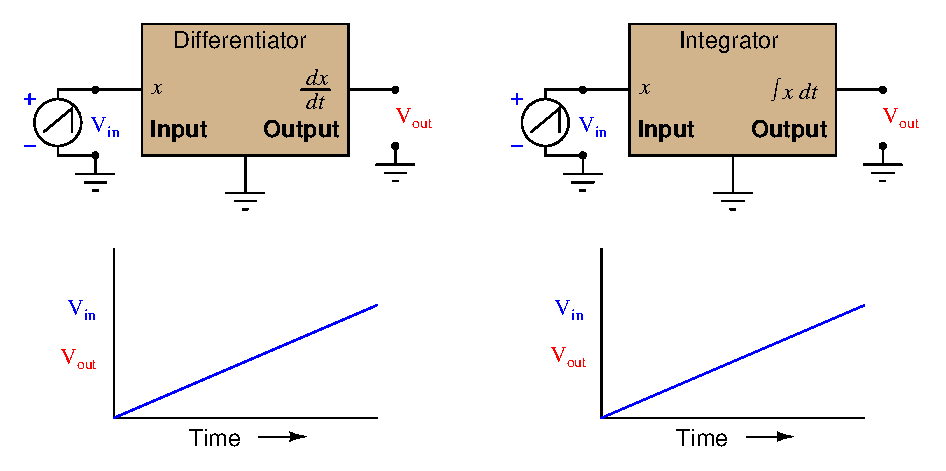
\includegraphics[width=15.5cm]{i01571x01.eps}$$

\vskip 20pt \vbox{\hrule \hbox{\strut \vrule{} {\bf Forslag til sokratisk diskusjon} \vrule} \hrule}

\begin{itemize}
\item{} Finn praktiske anvendelser i industrien for slike kretser.
\item{} Forklar hva som måtte være annerledes med inngangssignalet til hver krets for å generere en {\it negativ} utgangsspenning.
\item{} Forklar hvordan hver av disse kretsene vil respondere på et sinusformet inngangssignal med konstant frekvens.
\item{} Forklar hvordan hver av disse kretsene vil respondere på et sinusformet inngangssignal med økende frekvens.
\item{} Forklar hva som skjer dersom utgangen fra integratoren kobles til inngangen på derivereren, og et signal legges inn på integratoren. Hvilken type signal kommer ut av derivereren?
\item{} Forklar hva som skjer dersom utgangen fra derivereren kobles til inngangen på integratoren, og et signal legges inn på derivereren. Hvilken type signal kommer ut av integratoren?
\end{itemize}

\underbar{file i01571}
%(END_QUESTION)





%(BEGIN_ANSWER)

$$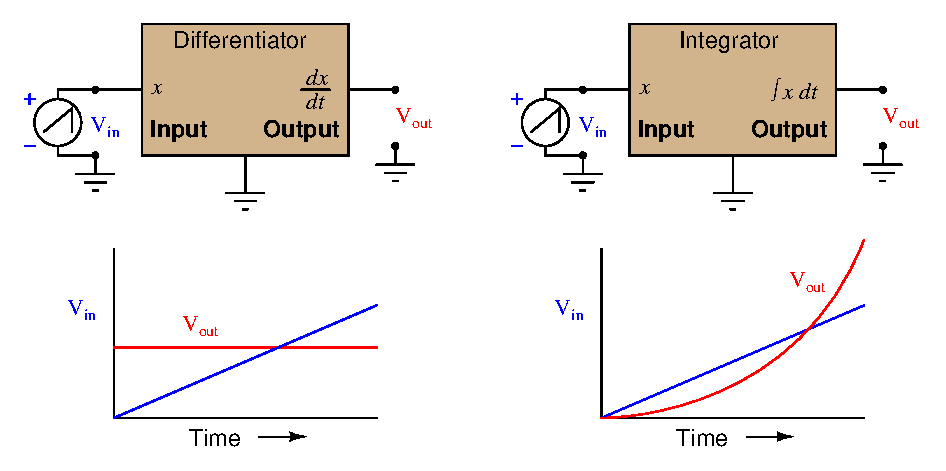
\includegraphics[width=15.5cm]{i01571x02.eps}$$

%(END_ANSWER)





%(BEGIN_NOTES)

Be studentene sette svarene sine inn i en praktisk sammenheng, for eksempel hastighet og strekning for et objekt i bevegelse (der hastighet er den tidsderiverte av strekning, og strekning er tidsintegralet av hastighet).

%INDEX% Electronics review: differentiator circuit response
%INDEX% Electronics review: integrator circuit response

%(END_NOTES)
